\documentclass[aspectratio=169,10pt]{beamer}

\usetheme{default}
\usecolortheme{default}
\usefonttheme{professionalfonts}

\usepackage[T1]{fontenc}
\usepackage[utf8]{inputenc}
\usepackage{lmodern}
\usepackage{amsmath,amssymb,mathtools,bm}
\usepackage{booktabs}
\usepackage{array}
\usepackage{graphicx}
\usepackage{tikz}
\usepackage[most]{tcolorbox}
\usetikzlibrary{arrows.meta,calc,patterns}

\definecolor{rtgnavy}{RGB}{12,35,64}
\definecolor{rtgorange}{RGB}{232,119,34}
\definecolor{rtgblue}{RGB}{59,124,184}
\definecolor{rtgred}{RGB}{184,86,69}
\definecolor{rtggreen}{RGB}{0,130,80}
\definecolor{rtggold}{RGB}{202,154,37}
\definecolor{rtggray}{RGB}{110,110,110}
\definecolor{rtglight}{RGB}{247,248,252}
\definecolor{rtgline}{RGB}{214,221,227}

\setbeamersize{text margin left=0.55cm,text margin right=0.55cm}
\setbeamertemplate{navigation symbols}{}
\setbeamertemplate{itemize item}{\textcolor{rtgorange}{\scriptsize$\blacktriangleright$}}
\setbeamertemplate{itemize subitem}{\textcolor{rtgnavy}{\tiny$\blacktriangleright$}}
\setbeamertemplate{enumerate item}{\textcolor{rtgnavy}{\insertenumlabel.}}
\setbeamercolor{normal text}{fg=rtgnavy,bg=white}
\setbeamercolor{frametitle}{fg=rtgnavy}
\setbeamercolor{structure}{fg=rtgnavy}
\setbeamercolor{alerted text}{fg=rtgorange}
\setbeamercolor{footline}{fg=rtggray}
\setbeamerfont{frametitle}{series=\bfseries,size=\large}
\setbeamerfont{footline}{size=\tiny}
\setbeamerfont{title}{series=\bfseries,size=\Large}
\setbeamerfont{subtitle}{size=\small}

\setbeamertemplate{footline}{%
  \hfill
  \usebeamerfont{footline}\usebeamercolor[fg]{footline}%
  \insertshortauthor\quad|\quad\insertshorttitle
  \quad|\quad\insertframenumber/\inserttotalframenumber
  \hspace{1em}\vspace{0.35em}
}

\setbeamertemplate{frametitle}{%
  \vspace{0.25em}%
  \usebeamerfont{frametitle}\usebeamercolor[fg]{frametitle}%
  \insertframetitle\par
  \vspace{0.05em}%
  {\color{rtgorange}\hrule height 0.8pt}%
  \vspace{0.12em}%
}

\setlength{\leftmargini}{1.15em}
\setlength{\leftmarginii}{1.0em}
\setlength{\abovedisplayskip}{5pt}
\setlength{\belowdisplayskip}{5pt}
\setlength{\abovedisplayshortskip}{3pt}
\setlength{\belowdisplayshortskip}{3pt}

\tcbset{
  slideboxA/.style={
    colback=rtglight,colframe=rtgnavy,
    fonttitle=\small\bfseries,
    top=3pt,bottom=3pt,left=4pt,right=4pt,boxsep=0pt
  },
  slideboxB/.style={
    colback=rtglight,colframe=rtgorange,
    fonttitle=\small\bfseries,
    top=3pt,bottom=3pt,left=4pt,right=4pt,boxsep=0pt
  },
  slideboxC/.style={
    colback=rtglight,colframe=rtggreen,
    fonttitle=\small\bfseries,
    top=3pt,bottom=3pt,left=4pt,right=4pt,boxsep=0pt
  }
}

\title[Higher-Dimensional Parameter Collapse]{Parameter Collapse in Higher Dimensions}
\subtitle{A Visual and Experimental Plan for Open Problem 4.2}
\author[NSF RTG Project 4]{NSF RTG Project 4}
\institute{Auburn University}
\date{June 5, 2026}

\begin{document}

{
\setbeamertemplate{footline}{}
\setbeamertemplate{frametitle}{}
\begin{frame}
  \begin{tikzpicture}[remember picture,overlay]
    \fill[rtgnavy] (current page.south west) rectangle (current page.north east);
    \fill[rtgorange] (current page.south west) rectangle ([yshift=0.48cm]current page.south east);
  \end{tikzpicture}
  \vspace{1.75cm}
  \begin{center}
    {\color{white}\bfseries\Large Parameter Collapse in Higher Dimensions}\\[0.28cm]
    {\color{white!85}\small A Visual and Experimental Plan for Open Problem 4.2}\\[0.55cm]
    {\color{white}NSF RTG Project 4}\\[0.20cm]
    {\color{white!85}\small Auburn University}\\[0.20cm]
    {\color{white!85}June 5, 2026}
  \end{center}
\end{frame}
}

\begin{frame}{Motivation and Open Problem 4.2}
\small
\begin{columns}[T,onlytextwidth]
\column{0.49\textwidth}
\textbf{\textcolor{rtgnavy}{The 1D phenomenon}}
\begin{itemize}
  \item In one dimension, each ReLU neuron places a \textbf{kink point} at $b_j$.
  \item During gradient flow, many $b_j$ appear to merge into a small number of clusters.
  \item This reduces the effective number of neurons without explicit pruning.
\end{itemize}

\vspace{0.08cm}
\begin{center}
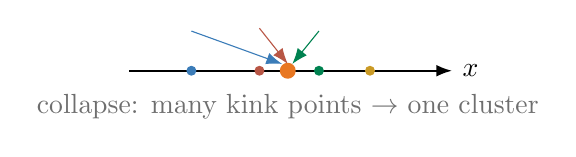
\begin{tikzpicture}[scale=0.72]
  \draw[-{Latex[length=2mm]},thick] (-2.8,0) -- (2.9,0) node[right] {$x$};
  \foreach \x/\col in {-1.7/rtgblue,-0.5/rtgred,0.55/rtggreen,1.45/rtggold}
    \fill[\col] (\x,0) circle (2.5pt);
  \draw[-{Latex[length=2mm]},rtgblue] (-1.7,0.7) -- (-0.1,0.12);
  \draw[-{Latex[length=2mm]},rtgred] (-0.5,0.75) -- (0.0,0.12);
  \draw[-{Latex[length=2mm]},rtggreen] (0.55,0.7) -- (0.08,0.12);
  \fill[rtgorange] (0,0) circle (4pt);
  \node[below,rtggray] at (0,-0.25) {collapse: many kink points $\to$ one cluster};
\end{tikzpicture}
\end{center}

\column{0.47\textwidth}
\textbf{\textcolor{rtgnavy}{Higher-dimensional question}}
\[
f(x)=\sum_{j=1}^m a_j\sigma(w_j^\top x+b_j),\qquad x\in\mathbb{R}^d .
\]
\begin{itemize}
  \item In $\mathbb{R}^d$, the kink is no longer a point.
  \item Each neuron defines a hyperplane:
  \[
  \{x:w_j^\top x+b_j=0\}.
  \]
  \item Open Problem 4.2 asks whether collapse generalizes to configurations of these hyperplanes.
\end{itemize}

\vspace{0.08cm}
\begin{tcolorbox}[slideboxA]
\centering\textbf{Goal:} make the 2D and 3D geometry explicit.
\end{tcolorbox}
\end{columns}
\end{frame}

\begin{frame}{Geometry Dictionary: Point, Line, Plane}
\small
\begin{columns}[T,onlytextwidth]
\column{0.31\textwidth}
\textbf{\textcolor{rtgblue}{$d=1$: kink point}}
\[
x-b_j=0
\]
\begin{center}
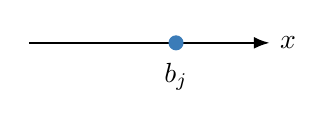
\begin{tikzpicture}[scale=0.68]
  \draw[-{Latex[length=2mm]},thick] (-2.2,0) -- (2.3,0) node[right] {$x$};
  \fill[rtgblue] (0.55,0) circle (4pt);
  \node[below] at (0.55,-0.2) {$b_j$};
\end{tikzpicture}
\end{center}
\small Only a location must be tracked.

\column{0.31\textwidth}
\textbf{\textcolor{rtgred}{$d=2$: kink line}}
\[
w_j^\top x+b_j=0
\]
\begin{center}
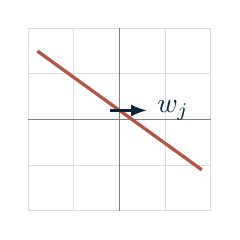
\begin{tikzpicture}[scale=0.58]
  \draw[rtgline] (-2,-2) grid (2,2);
  \draw[gray] (-2,0) -- (2,0);
  \draw[gray] (0,-2) -- (0,2);
  \draw[rtgred,very thick] (-1.8,1.5) -- (1.8,-1.1);
  \draw[-{Latex[length=2mm]},rtgnavy,thick] (-0.2,0.2) -- (0.6,0.2) node[right] {$w_j$};
\end{tikzpicture}
\end{center}
\small Track orientation and offset.

\column{0.31\textwidth}
\textbf{\textcolor{rtggreen}{$d=3$: kink plane}}
\[
w_j^\top x+b_j=0
\]
\begin{center}
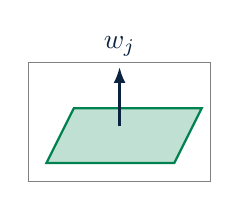
\begin{tikzpicture}[scale=0.58]
  \coordinate (A) at (-1.6,-0.8);
  \coordinate (B) at (1.2,-0.8);
  \coordinate (C) at (1.8,0.4);
  \coordinate (D) at (-1.0,0.4);
  \fill[rtggreen!25] (A)--(B)--(C)--(D)--cycle;
  \draw[rtggreen,thick] (A)--(B)--(C)--(D)--cycle;
  \draw[-{Latex[length=2mm]},rtgnavy,thick] (0,0) -- (0,1.3) node[above] {$w_j$};
  \draw[gray] (-2,-1.2) rectangle (2,1.4);
\end{tikzpicture}
\end{center}
\small Track normal direction and offset.
\end{columns}

\vspace{0.12cm}
\centering
\begin{tcolorbox}[slideboxB,width=0.88\textwidth]
\centering\textbf{Main change:} higher-dimensional collapse can occur in orientation, offset, or both.
\end{tcolorbox}
\end{frame}

\begin{frame}{Why Normalize by $\|w_j\|$?}
\small
\begin{columns}[T,onlytextwidth]
\column{0.49\textwidth}
\textbf{\textcolor{rtgnavy}{Raw bias is not geometric displacement}}

\vspace{0.05cm}
A hyperplane is unchanged if both $w_j$ and $b_j$ are multiplied by the same nonzero scalar.

\vspace{0.08cm}
\[
x_1-0.4=0
\qquad\text{and}\qquad
2x_1-0.8=0
\]
represent the same line, but the raw bias changes.

\begin{center}
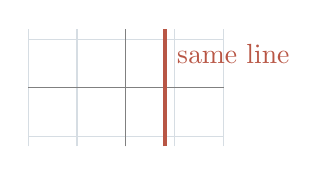
\begin{tikzpicture}[scale=0.62]
  \draw[rtgline] (-2,-1.2) grid (2,1.2);
  \draw[gray] (-2,0) -- (2,0);
  \draw[gray] (0,-1.2) -- (0,1.2);
  \draw[rtgred,very thick] (0.8,-1.2) -- (0.8,1.2);
  \node[rtgred,right] at (0.85,0.7) {same line};
\end{tikzpicture}
\end{center}

\column{0.47\textwidth}
\textbf{\textcolor{rtgnavy}{Canonical hyperplane variables}}
\[
n_j=\frac{w_j}{\|w_j\|},
\qquad
\beta_j=\frac{b_j}{\|w_j\|}.
\]
\begin{itemize}
  \item $n_j$ is the unit normal direction.
  \item $\beta_j$ is the signed offset from the origin.
  \item These variables remove arbitrary scaling.
  \item In 2D, $n_j$ can be summarized by an angle $\theta_j$, so each neuron becomes a point $(\theta_j,\beta_j)$.
\end{itemize}
\end{columns}
\end{frame}

\begin{frame}{2D Case A: Ridge Targets Force Directional Collapse}
\small
\[
f^\ast(x)=\sin(2\pi u^\top x)+0.5\sin(4\pi u^\top x).
\]
\vspace{-0.35cm}
Take $u=(1,0)$. Then $u^\top x=x_1$, so the target varies only in the horizontal direction.

\begin{columns}[T,onlytextwidth]
\column{0.49\textwidth}
\begin{center}
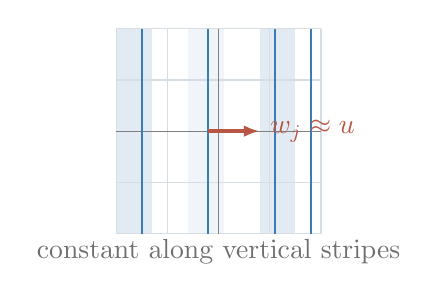
\begin{tikzpicture}[scale=0.65]
  \fill[rtgblue!15] (-2,-2) rectangle (-1.3,2);
  \fill[rtgblue!8] (-0.6,-2) rectangle (0.1,2);
  \fill[rtgblue!15] (0.8,-2) rectangle (1.5,2);
  \draw[rtgline] (-2,-2) grid (2,2);
  \draw[gray] (-2,0) -- (2,0);
  \draw[gray] (0,-2) -- (0,2);
  \foreach \x in {-1.5,-0.2,1.1,1.8}
    \draw[rtgblue,thick] (\x,-2) -- (\x,2);
  \draw[-{Latex[length=2mm]},rtgred,very thick] (-0.2,0) -- (0.8,0) node[right] {$w_j\approx u$};
  \node[rtggray] at (0,-2.35) {constant along vertical stripes};
\end{tikzpicture}
\end{center}

\column{0.47\textwidth}
\textbf{\textcolor{rtgnavy}{Expected collapse pattern}}
\begin{itemize}
  \item The function changes only along $u$.
  \item Useful neurons should have normals $w_j$ aligned with $u$.
  \item Their hyperplane lines are therefore approximately perpendicular to $u$.
\end{itemize}

\vspace{0.08cm}
\begin{tcolorbox}[slideboxA]
\centering\textbf{Prediction:} angular entropy decreases and $\theta_j$ clusters near the direction of $u$.
\end{tcolorbox}

\vspace{0.08cm}
\small\textit{Important: the normal vectors collapse toward $u$; the lines themselves are perpendicular to $u$.}
\end{columns}
\end{frame}

\begin{frame}{2D Case B: Separable Targets Produce Direction Families}
\small
\[
f^\ast(x)=\sin(2\pi x_1)+\sin(2\pi x_2).
\]
\vspace{-0.25cm}
This target is the sum of one structure in $x_1$ and one structure in $x_2$.

\begin{columns}[T,onlytextwidth]
\column{0.49\textwidth}
\begin{center}
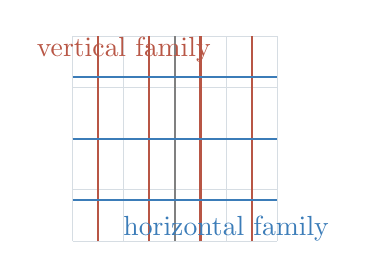
\begin{tikzpicture}[scale=0.65]
  \draw[rtgline] (-2,-2) grid (2,2);
  \draw[gray] (-2,0) -- (2,0);
  \draw[gray] (0,-2) -- (0,2);
  \foreach \x in {-1.5,-0.5,0.5,1.5}
    \draw[rtgred,thick] (\x,-2) -- (\x,2);
  \foreach \y in {-1.2,0,1.2}
    \draw[rtgblue,thick] (-2,\y) -- (2,\y);
  \node[rtgred] at (-1.0,1.75) {vertical family};
  \node[rtgblue] at (1.0,-1.75) {horizontal family};
\end{tikzpicture}
\end{center}

\column{0.47\textwidth}
\textbf{\textcolor{rtgnavy}{Expected collapse pattern}}
\begin{itemize}
  \item One group of neurons learns variation along $x_1$.
  \item Another group learns variation along $x_2$.
  \item The hyperplanes do not all collapse to one direction; they form two interpretable families.
\end{itemize}

\vspace{0.08cm}
\begin{tcolorbox}[slideboxB]
\centering\textbf{Prediction:} the $\theta_j$ distribution becomes bimodal, with one mode for each coordinate direction.
\end{tcolorbox}
\end{columns}
\end{frame}

\begin{frame}{2D Case C: Radial Targets Resist Single-Direction Collapse}
\small
\[
f^\ast(x)=\cos(\pi\|x\|).
\]
\vspace{-0.25cm}
This target depends on distance from the origin, not on one fixed direction.

\begin{columns}[T,onlytextwidth]
\column{0.49\textwidth}
\begin{center}
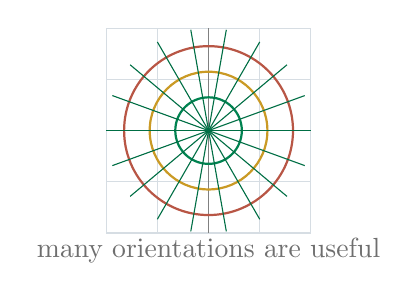
\begin{tikzpicture}[scale=0.65]
  \draw[rtgline] (-2,-2) grid (2,2);
  \draw[gray] (-2,0) -- (2,0);
  \draw[gray] (0,-2) -- (0,2);
  \draw[rtggreen,thick] (0,0) circle (0.65);
  \draw[rtggold,thick] (0,0) circle (1.15);
  \draw[rtgred,thick] (0,0) circle (1.65);
  \foreach \a in {0,20,...,160}
    \draw[rtggreen!85!black] ({-2*cos(\a)},{-2*sin(\a)}) -- ({2*cos(\a)},{2*sin(\a)});
  \node[rtggray] at (0,-2.35) {many orientations are useful};
\end{tikzpicture}
\end{center}

\column{0.47\textwidth}
\textbf{\textcolor{rtgnavy}{Expected collapse pattern}}
\begin{itemize}
  \item No single direction $u$ explains the target.
  \item A good approximation may require many tangent-like directions.
  \item Collapse may still occur locally, but full directional collapse is unlikely.
\end{itemize}

\vspace{0.08cm}
\begin{tcolorbox}[slideboxC]
\centering\textbf{Prediction:} offsets may cluster, but angular entropy remains higher than in the ridge case.
\end{tcolorbox}
\end{columns}
\end{frame}

\begin{frame}{3D Cases: Collapse of Planes}
\small
\begin{columns}[T,onlytextwidth]
\column{0.31\textwidth}
\textbf{\textcolor{rtgred}{Same plane}}
\begin{center}
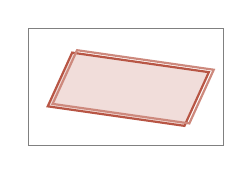
\begin{tikzpicture}[scale=0.62]
  \fill[rtgred!20] (-1.6,-0.4)--(1.2,-0.8)--(1.7,0.3)--(-1.1,0.7)--cycle;
  \draw[rtgred,thick] (-1.6,-0.4)--(1.2,-0.8)--(1.7,0.3)--(-1.1,0.7)--cycle;
  \draw[rtgred!70,thick] (-1.5,-0.35)--(1.3,-0.75)--(1.8,0.35)--(-1.0,0.75)--cycle;
  \draw[gray] (-2,-1.2) rectangle (2,1.2);
\end{tikzpicture}
\end{center}
\small $n_j$ and $\beta_j$ both cluster.

\column{0.31\textwidth}
\textbf{\textcolor{rtgblue}{Parallel planes}}
\begin{center}
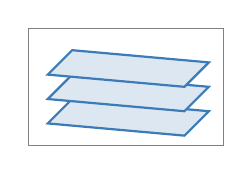
\begin{tikzpicture}[scale=0.62]
  \foreach \y in {-0.75,-0.25,0.25} {
    \fill[rtgblue!18] (-1.6,\y)--(1.2,\y-0.25)--(1.7,\y+0.25)--(-1.1,\y+0.5)--cycle;
    \draw[rtgblue,thick] (-1.6,\y)--(1.2,\y-0.25)--(1.7,\y+0.25)--(-1.1,\y+0.5)--cycle;
  }
  \draw[gray] (-2,-1.2) rectangle (2,1.2);
\end{tikzpicture}
\end{center}
\small $n_j$ clusters but $\beta_j$ differs.

\column{0.31\textwidth}
\textbf{\textcolor{rtggreen}{Direction families}}
\begin{center}
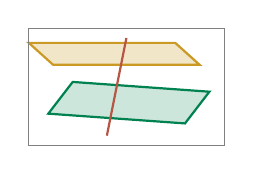
\begin{tikzpicture}[scale=0.62]
  \fill[rtggreen!20] (-1.6,-0.55)--(1.2,-0.75)--(1.7,-0.1)--(-1.1,0.1)--cycle;
  \draw[rtggreen,thick] (-1.6,-0.55)--(1.2,-0.75)--(1.7,-0.1)--(-1.1,0.1)--cycle;
  \fill[rtggold!25] (-1.5,0.45)--(1.5,0.45)--(1.0,0.9)--(-2.0,0.9)--cycle;
  \draw[rtggold,thick] (-1.5,0.45)--(1.5,0.45)--(1.0,0.9)--(-2.0,0.9)--cycle;
  \draw[rtgred,thick] (-0.4,-1.0)--(0.0,1.0);
  \draw[gray] (-2,-1.2) rectangle (2,1.2);
\end{tikzpicture}
\end{center}
\small Several normal directions persist.
\end{columns}

\vspace{0.12cm}
\centering
\begin{tcolorbox}[slideboxB,width=0.90\textwidth]
\centering 3D adds geometric richness: collapse may reduce planes to one plane, parallel stacks, or a few normal-direction families.
\end{tcolorbox}
\end{frame}

\begin{frame}{Experimental Protocol and Diagnostics}
\small
\begin{columns}[T,onlytextwidth]
\column{0.49\textwidth}
\textbf{\textcolor{rtgnavy}{Protocol}}
\begin{enumerate}
  \item \textbf{Train:} run gradient flow for a shallow ReLU network on $[-1,1]^2$ or $[-1,1]^3$.
  \item \textbf{Normalize:} convert each neuron to $(n_j,\beta_j)$.
  \item \textbf{Cluster:} in 2D, cluster $(\theta_j,\beta_j)$; in 3D, cluster normal directions and offsets.
  \item \textbf{Prune:} merge neurons inside each cluster and compare loss before and after pruning.
\end{enumerate}

\column{0.47\textwidth}
\textbf{\textcolor{rtgnavy}{Diagnostics}}
\begin{itemize}
  \item \textbf{Angular entropy:} does the direction distribution concentrate?
  \item \textbf{Offset clusters:} do $\beta_j$ values merge inside a direction family?
  \item \textbf{Effective width:} how many clusters remain after training?
  \item \textbf{Pruning gap:} does cluster merging preserve test error?
\end{itemize}

\vspace{0.08cm}
\begin{tcolorbox}[slideboxA]
\centering\textbf{Evidence for OP 4.2} is not just fewer neurons. It is stable geometric concentration plus successful pruning.
\end{tcolorbox}
\end{columns}
\end{frame}

\begin{frame}{Expected Outcomes and Research Direction}
\small
\textbf{\textcolor{rtgnavy}{Target-dependent predictions}}

\vspace{0.05cm}
\begin{center}
\resizebox{0.96\textwidth}{!}{%
\begin{tabular}{lll}
\toprule
\textbf{Case} & \textbf{Expected geometry} & \textbf{Collapse mode}\\
\midrule
Ridge & one dominant normal direction & directional collapse\\
Separable & two coordinate families & family collapse\\
Radial & many useful orientations & partial or local collapse\\
3D structured & planes organize by normals and offsets & plane-family collapse\\
\bottomrule
\end{tabular}
}
\end{center}

\vspace{0.12cm}
\begin{columns}[T,onlytextwidth]
\column{0.54\textwidth}
\textbf{\textcolor{rtgnavy}{Conjectural picture}}
\begin{itemize}
  \item Higher-dimensional collapse should be measured in hyperplane space, not only in raw parameters.
  \item The support may concentrate to points, curves, stacks of parallel hyperplanes, or several direction families.
\end{itemize}

\column{0.42\textwidth}
\textbf{\textcolor{rtgnavy}{Next deliverable}}
\vspace{0.05cm}
\begin{tcolorbox}[slideboxB]
Run the three 2D cases, plot $(\theta_j,\beta_j)$ over time, and test whether pruning after clustering preserves loss.
\end{tcolorbox}
\end{columns}
\end{frame}

\end{document}
